%%%%%%%%%%%%%%%%%%%%%%%%%%%%%%%%%%%%%%%%%%%%%%
%%%%%%%%%%%%%%%%%%%%%%%%%%%%%%%%%%%%%%%%%%%%%%
%%% Master Thesis Template by Fabian Schär %%%
%%%%%%%%%%%%%%%%%%%%%%%%%%%%%%%%%%%%%%%%%%%%%%
%%%%%%%%%%%%%%%%%%%%%%%%%%%%%%%%%%%%%%%%%%%%%%

%%%%%%%%%%%%%%%%%%%%%%%%%%%%%%%%%%%%%%
%%% Packages and Document Settings %%%
%%%%%%%%%%%%%%%%%%%%%%%%%%%%%%%%%%%%%%

\documentclass[12pt,a4paper,titlepage,oneside,english]{article}

%%% Main Packages %%%
\usepackage[english]{babel}
%\usepackage[ngerman]{babel} % Use this option for German settings.
\usepackage[T1]{fontenc}
\usepackage[utf8]{inputenc}

%%% Additional Packages %%%
\usepackage{cite}
\usepackage{framed}
\usepackage{graphicx}
%\usepackage[german]{fancyref}
%\usepackage[german,hidelinks]{hyperref} %hidelinks
\usepackage{multirow}
\usepackage[round]{natbib}
\usepackage{setspace}
\usepackage{geometry}
\usepackage{pst-all} % Not working with Sweave!!!
\usepackage{hyperref}
\usepackage[nobiblatex]{xurl}

%%% Math Packages %%%
\usepackage{amsmath}
\usepackage{amstext}
\usepackage{amssymb}
\usepackage{theorem}
\usepackage{epsfig}
\usepackage{longtable}
\usepackage[lined, commentsnumbered, ruled]{algorithm2e}
\usepackage{listings}

%%% Layout Specifications %%%
\geometry{a4paper, top=35mm, left=40mm, right=40mm, bottom=45mm,
headsep=10mm, footskip=12mm}

%%% Tikz Styles %%%
\usepackage{tikz}
\usetikzlibrary{backgrounds}
\usetikzlibrary{arrows}
\usetikzlibrary{shapes,shapes.geometric,shapes.misc}

% this style is applied by default to any tikzpicture included via \tikzfig
\tikzstyle{tikzfig}=[baseline=-0.25em,scale=0.5]

% these are dummy properties used by TikZiT, but ignored by LaTex
\pgfkeys{/tikz/tikzit fill/.initial=0}
\pgfkeys{/tikz/tikzit draw/.initial=0}
\pgfkeys{/tikz/tikzit shape/.initial=0}
\pgfkeys{/tikz/tikzit category/.initial=0}

% standard layers used in .tikz files
\pgfdeclarelayer{edgelayer}
\pgfdeclarelayer{nodelayer}
\pgfsetlayers{background,edgelayer,nodelayer,main}

% style for blank nodes
\tikzstyle{none}=[inner sep=0mm]

% include a .tikz file
\newcommand{\tikzfig}[1]{%
{\tikzstyle{every picture}=[tikzfig]
\IfFileExists{#1.tikz}
  {\input{#1.tikz}}
  {%
    \IfFileExists{./figures/#1.tikz}
      {\input{./figures/#1.tikz}}
      {\tikz[baseline=-0.5em]{\node[draw=red,font=\color{red},fill=red!10!white] {\textit{#1}};}}%
  }}%
}

% the same as \tikzfig, but in a {center} environment
\newcommand{\ctikzfig}[1]{%
\begin{center}\rm
  \tikzfig{#1}
\end{center}}

% fix strange self-loops, which are PGF/TikZ default
\tikzstyle{every loop}=[]

\input{../assetlib/tikz/styles.tikzstyles}

%%% Parskip Settings %%%
\setlength{\parskip}{3mm}
\setlength{\parindent}{0mm}

%%% Document Specifications %%%
\title{A solidity smart contract for rental deposit accounts}
\author{Matthias Nadler}


%%%%%%%%%%%%%%%%%%
%%% Title Page %%%
%%%%%%%%%%%%%%%%%%

\begin{document}
%\begin{titlepage}
\begin{center}
\vspace{1em}
%\large{Seminar Paper}\\
%\large{Bachelor Thesis}\\
\large{Seminar Thesis}\\
\huge A solidity smart contract \\
for rental deposit accounts \\
\Large \vspace{1em}
Matthias Nadler
\end{center}

\vspace{1em}
\normalsize
\begin{flushleft}
Supervised by:\\ 
Prof. Dr. Fabian Schär \\
Credit Suisse Asset Management (Schweiz) Professor for \\ 
Distributed Ledger Technologies and Fintech \\
Center for Innovative Finance, University of Basel
\end{flushleft}

\vspace{1em}
\onehalfspacing
\begin{center}
\section*{Abstract}
\end{center}
We present a smart contract version of a rental deposit account on the Ethereum blockchain. The deposited security, provided in the form of DAI, is securely invested while remaining under control of the smart contract, generating interest for the tenant. The analysis of incentives and risks for the participants indicate that a blockchain-based, digital form of contracts can be successful, if enough trust is placed in the underlying technologies and if they are paired with traditional, off-chain contracts.

\vfill
\textbf{Keywords:} Ethereum, smart contract, DAI, rental deposit account.\\
\noindent\textbf{JEL:} G21, G52, G19
%\end{titlepage}


%%%%%%%%%%%%%%%%%%%%%%%%%%%%%%%%%%%%%%%%
%%% Inhaltsverzeichnis & Plagiatserklärung
%%%%%%%%%%%%%%%%%%%%%%%%%%%%%%%%%%%%%%%%

\pagenumbering{gobble}

\newpage
\pagenumbering{Roman}
\tableofcontents
\vfill
\begin{center}
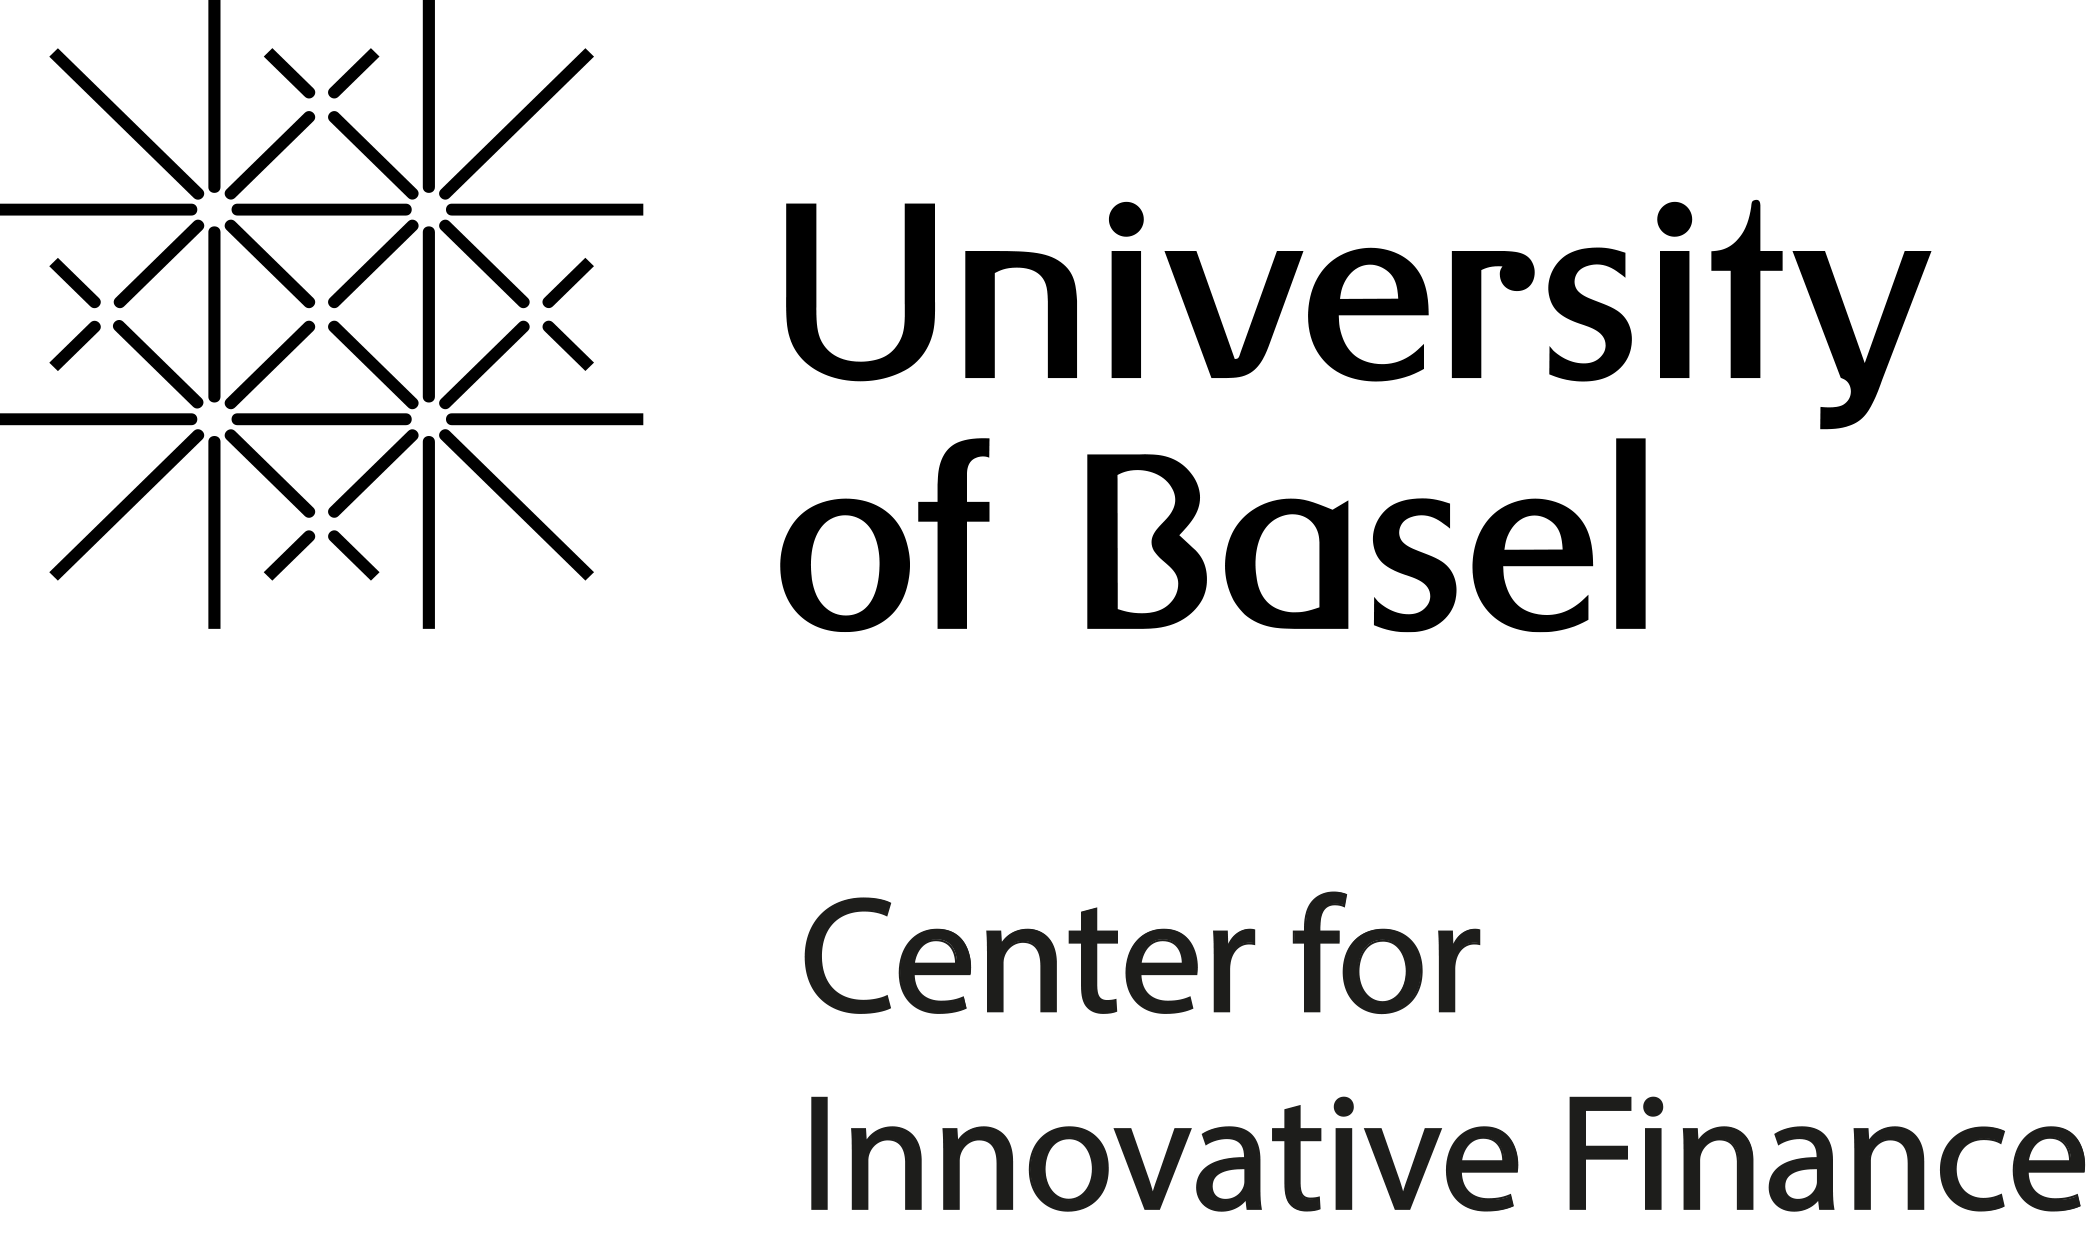
\includegraphics[width=4cm]{../assetlib/images/logo_cif.png}
\end{center}
\singlespacing
\vspace{-1.5cm}
\section*{Plagiatserklärung}
Ich bezeuge mit meiner Unterschrift, dass meine Angaben über die bei der Abfassung meiner Arbeit benutzten Hilfsmittel sowie über die mir zuteil gewordene Hilfe in jeder Hinsicht der Wahrheit entsprechen und vollständig sind. Ich habe das Merkblatt zu Plagiat und Betrug vom 22. Februar 2011 gelesen und bin mir der Konsequenzen eines solchen Handelns bewusst.\\

%% YOUR NAME HERE %%
Matthias Nadler
%%%%%%%%%%%%%%%%%%%%

\newpage
\onehalfspacing
\pagenumbering{arabic}


%%%%%%%%%%%%%%%%%%%%%%%%%%%%%%%%%%%%%%%%
%%% Introduction
%%%%%%%%%%%%%%%%%%%%%%%%%%%%%%%%%%%%%%%%

\section{Introduction}
\label{sec:introduction}
In Switzerland, according to the code of obligations (\textit{dt. Obligationenrecht, OR})  Art. 257e para. 1, a rental deposit needs to be placed in a (savings-) account at a bank, or in a deposit on the tenants name. The interest rate for a rental deposit account at one of Switzerland's largest three banks is between 0\% (UBS, Credit Suisse) and 0.05\% (Raiffeisen).\footnote{As of March 8th 2020, according to the official rates published by the banks.}

Setup, changes and release or restitution related to the deposit account all have to be handled in paper forms and require the signatures of both the tenant and the renter. These are time consuming processes for all involved parties.

The presented rental deposit account (short: RDA) smart contract attempts to solve both problems, allowing for higher interest rates for the tenant and for immediate, digital and secure transactions between the parties. 

\subsection{Smart Contracts}
\label{sub:smart-contracts}
Smart contracts are similar to traditional contracts, but they are written in a computer language and deployed on a system that is accessible to all contract parties. When interacting with a smart contract program or protocol, the code is able verify your instructions and enforce the resulting actions.

There are a few issues and questions that arise with the implementation of smart contracts. Most of these can be elegantly solved by deploying the smart contract on a public blockchain\footnote{It is assumed that the reader is familiar with blockchain and accompanying terminology. For an in-depth introduction to the topic the author recommends \cite{Schaer2017} (in German) or \cite{Lewis2018} (in English).} with a Turing complete language\footnote{A touring complete programming language has all the necessary instructions to solve any computational problem given enough resources. Bitcoin for example does not have a touring complete language, therefore no universal smart contracts can be deployed on this blockchain.}.


\begin{description}
	\item[Availability] A public blockchain is always online and accessible from everywhere. Each smart contract is deployed at a fixed address on the blockchain.
	\item[Authentication] Blockchains use private key cryptography to guarantee ownership of accounts. Smart contracts need no additional authentication logic.
	\item[Immutability] The most difficult feature to replicate without a public blockchain. The code of a deployed smart contract can never be changed. This means no one has the ability to alter the contract retroactively. Often times this also removes the need for a third party trustee and makes completely trust-less interactions possible.
	\item[Power to enforce] Smart contracts, like any other address, can directly control digital assets built on top of the blockchain. Any coin or token sent to a contract can not be recovered  unless it is transferred by the contract logic.
	\item[Transparency] The full contract code and every past interaction with the smart contract is stored on the blockchain and publicly available.
\end{description}

Our rental deposit account will combine a smart contract as described above with traditional off-chain contracts to create a more efficient agreement between the involved parties.

\subsection{Ethereum}
\label{sub:ethereum}

Any blockchain that implements a Turing complete programming language can be used to develop smart contracts. Among these options, Ethereum is the most popular according to an ecosystem report by \cite{ElectricCapital2019}: Of all open source crypto developers, 18\% worked in the Ethereum ecosystem during the first half of 2019. This is around four times more than for the second most popular platform EOS.

More reasons to develop this project on Ethereum include: The University of Basel teaches Solidity - the Ethereum specific programming language - in their courses. Ethereum has the widest array of decentralized finance products, including a very successful stablecoin which is the cornerstone of our application. Finally, the shortcomings of Ethereum compared to its alternatives - fewer transactions per second and higher transaction costs - are mitigated since our contract will perform very few transactions over its lifetime.



%%%%%%%%%%%%%%%%%%
%%% Incentives %%%
%%%%%%%%%%%%%%%%%%

\section{Improving rental deposit accounts}
In this section we will give a short overview of how a smart RDA contract operates and then take a look at the distribution of incentives, obligations and risks for each of the three parties in a traditional rental deposit account contract and how these aspects change for the smart contract variant.
It is assumed the reader is familiar on a basic level with the workings of smart contracts on the Ethereum blockchain.

\subsection{Smart RDA Contract}
A smart RDA contract can be created by anyone for a small transaction fee. To create it, one has to specify immutable Ethereum addresses for the three involved parties: Tenant, landlord and trustee; as well as a fixed trustee fee. The tenant then transfers the full deposit amount in DAI - a crypto stablecoin\footnote{See the Maker whitepaper \cite{MakerWhitepaper}.} - to the contract and starts the contract with another transaction. This locks the DAI security in the DAI savings rate contract (short: DSR) and begins to generate compounding interest on the locked capital. The trustee fee is paid by the contract to the trustee using aggregated interest.
Figure \ref{fig:contract} shows a more detailed, schematic view of how the smart RDA works. Note that it is not possible to interact with the deposit directly, every action is delegated by the RDA smart contract. Actions shown with a dotted line require the consent of at least two participants before they can be executed, as described in section \ref{sec:multisig}.

\begin{figure}[h]
\ctikzfig{contract}
\caption{The smart RDA contract is in control}
\label{fig:contract}
\end{figure}

\subsection{The Trustee}
The recommendation by Swiss Law (OR Art. 257e para. 1) is to store the deposit in the form of money or other securities on a (savings-) bank account. The reason for using a bank as the trustee is to minimize the counterparty risk. The bank assumes the role of a trustee and guarantees to safe-keep the deposit until it is eventually released to the tenant or landlord. According to OR Art. 257e para 3., the release of the deposit can be requested in a form signed by the tenant and the renter or with a legal instruction by a court or debt enforcement office. During the lifetime of the deposit, the bank is in full control; they can invest it and keep the earnings of this investment. As noted in section \ref{sec:introduction}, the interest passed on to the owner of the deposit is between 0\% and 0.05\% p.a. 

The smart rental deposit account contract still requires a trustee to trigger a release of the deposit to the right party if the tenant and the renter are not in agreement. But contrary to the traditional bank deposit, the counterparty risk is greatly mitigated by using a smart contract since the control over the funds will always remain with the contract and not the trustee.
For this reason, the role of the trustee can be assumed by any entity that both the tenant and the renter can agree upon: For example a notary or an institution that offers this service. A compensation has to be provided to the trustee to perform his services, but this compensation, called a trustee fee, can be in form of a one time fixed payment.

\subsection{The Tenant}
With a smart rental deposit contract the locked assets of the tenant are securely invested (while remaining under full control of the contract) and the tenant is eligible for any resulting earnings. On the other hand, the tenant has to pay the fixed trustee fee and assume all of the newly arising risks linked to the underlying technology described in section \ref{sec:risks}. As long as the interest rate of the DSR contract is sufficiently high, the renting period is sufficiently long (to offset the trustee fee) and the tenant values the risks of a system failure low enough, the smart deposit contract will provide a significant upgrade to the traditional system for the tenant.

\subsection{The Landlord}
Ideally, nothing would change for the landlord. However, the additional risks that arise by using a new and developing technology can not be fully absorbed by the tenant. A small risk remains for the renter: The underlying asset losing some or all of its value while the tenant at the same time becomes insolvent. 
To compensate for this, we suggest to increase the total amount of the deposit. For example use four instead of three month's worth of rent as the deposit. Note that this is much less detrimental for the tenant than it would be in a traditional setting, as the locked assets will be invested at a profit.

\subsection{Speed and Ease of settlements}
Interacting with a traditional rental deposit account poses significant transaction costs for all involved parties: Every action requires a written form with the signatures of the tenant and the landlord to be sent to the bank which can take days or weeks to complete. For the smart RDA, all these actions can be performed instantly online with a very small transaction fee \footnote{Transaction costs on the Ethereum blockchain are very volatile, but time-insensitive transactions can generally be executed for a few cents.}. If multiple signatures are needed for an action, that action can only be executed once the required parties have digitally agreed on the execution.

Authenticity of the signatures is guaranteed by the blockchain technology with the additional upside that any arbitrary document can be attached to an RDA and signed by the participants. This could for example be used to digitally sign the rental contract, eliminating the need for any physical documents and signatures in a tenant-renter relationship.


%%%%%%%%%%%%%%%%
%%% Risks    %%%
%%%%%%%%%%%%%%%%

\section{Risks}
\label{sec:risks}
In this section we discuss the most urgent risks that arise when using an RDA smart contract. The risks can be divided into Counterparty risk, foreign exchange risk and Layer 1 - Layer 4 risks as described by \cite{Schaer2020}. The following sections assume that the RDA smart contract works as intended; the risk of smart contract failure is covered in Layer 3 risks.

\subsection{Counterparty Risk}
As counterparty risk we understand the likelihood that one of the involved parties does not perform their contractual obligations, due to malicious intent or otherwise.
Most of the counterparty risk is mitigated by the smart contract nature of the RDA. Especially the funds are kept completely secure and can't be compromised. The obligations of the trustee - confirming multisig transactions when needed - need to be backed up by a written (off-chain) contract and there remains a risk that the trustee defaults on these obligations. However, the trustee has no personal gain from this behaviour and is contractually liable. It is still vital to chose a reputable entity for this task. Changing the trustee is possible if both the tenant and the landlord agree, but a new RDA needs to be set up.

The tenant or landlord can not behave in a way that will compromise the smart contract as long as the trustee fulfils their obligation.

\subsection{Foreign Exchange Risk}
Currently the only widely available stablecoins on the Ethereum platform are pegged to the US-Dollar; therefore the rental deposit needs to be paid in US-Dollar. If the US-Dollar is not the local currency of the country where the RDA contract is settled, there exists a risk for the deposit to become undercollateralized if the US-Dollar is devalued. This risk can be mitigated with hedging or similar strategies if desired, otherwise the tenant and the landlord need to agree to accept this risk. A further possibility would be to include a contract clause that will trigger a migration of the contract with re-collateralization should the exchange rate fall below a certain threshold.

\subsection{Settlement Layer Risk}
Layer 1 risks include a partial or total failure of the Ethereum protocol due to technical issues. This would most likely also default the entire rental deposit. The tenant is fully liable for this risk and needs to set up a new rental deposit on a different platform.

\subsection{Asset Layer Risk}
Layer 2 includes the assets built on the Ethereum protocol; relevant for this smart contract is the ERC-20 stablecoin DAI and by extension the MakerDAO ecosystem. MakerDAO is still very much a developing and experimental institution that brings the risk of a partial or complete failure. In most scenarios a total default can be prevented if the contract is migrated in time to a different platform on initiative of the trustee and the tenant. However, the tenant is responsible to re-collateralize the deposit. We try to keep the layer 2 risk minimal by not involving any other asset.

It is important to note that investing DAI by locking it in the DSR contract does not generate any additional risk. DSR deposits have guaranteed liquidity and no restrictions of any kind to retrieve the investment.

\subsection{Protocol Layer Risk}
The layer 3 risk is extensively described in \cite{Schaer2020}, section 3. It consists of smart contract execution risk (coding errors and vulnerabilities), operational security (OpSec) risks and dependency risks (dependency on MakerDao and especially DSR). 
OpSec risks are negligible as there exists no admin key for the smart contract. Execution risk and dependency risk is accepted by the tenant. One significant dependency risk is a low interest rate as defined by the DSR contract.

\subsection{Application Layer Risk}
The layer 4 risks arises if the parties decide to use the provided dApp at \url{https://smartdepos.it} or a similar external interface which has a chance to malfunction and submit faulty data to the RDA smart contract. Every participant bears this risk for themselves, but it is highest for the tenant as they need to send DAI transactions. The risk can be mitigated by interacting directly with the smart contract.


\section{Off-Chain Legal Contract}
A smart RDA contract should only be deployed with an additional off-chain legal contract between the parties. A draft for this document - in german and designed for the Swiss legislature - has been started in collaboration with a jurist consultant.

The document contains regulations for the following topics:
\begin{itemize}
	\item It ties the Ethereum addresses to a legal person, revealing their identity
	\item Guidelines for safekeeping the private keys to the used addresses and potential resulting consequences
	\item Representation by other parties in times of absence
	\item Detailed obligations of the involved parties, including rules for which participant is obligated to call and pay or confirm which actions on the contract
	\item Compensation for the trustee
	\item Incorporation into applicable Swiss contract law
	\item Situations that will trigger a deposit migration
	\item Taxation of interest profits
\end{itemize}

The document is not yet finished, but will be uploaded to the repository in the coming months.

%%%%%%%%%%%%%%%%
%%% Multisig %%%
%%%%%%%%%%%%%%%%

\section{Multisig on Ethereum}
\label{sec:multisig}
Multisig is the process when more than one account needs to sign a transaction before it can be executed. The Ethereum blockchain does not natively implement any multisig functionality unlike for example Bitcoin\footnote{Bitcoin's P2SH scheme (BIP16) can generate an address from any number of public keys with an additional parameter for how many signatures from these keys are needed for a transaction. This is implemented directly in the settlement layer and provides maximum security.}. Any implementation of multisig on Ethereum needs to be developed manually in a smart contract, which has been done by many different individuals and companies. However, these implementations are on the protocol layer, not the settlement layer and therefore much more prone to mistakes, bugs and vulnerabilities. The famous parity hacks of 2017 - see \cite{palladino2017parity} - were both caused by a careless implementation of the parity multisig wallet. It is therefore critical to build the multisig part of the RDA smart contract on a simple, understandable, verified and audited code base.


\subsection{Different Approaches to Multisig}
Signatures can be aggregated on-chain or off-chain and the content of the transaction can be stored on-chain or not. Which approach to use depends mostly on the use case of the contract.

\subsection{Off-Chain Implementation}
This implementation is the closest to how Bitcoin implements their multisig: A transaction is created off-chain and then sequentially signed by the required addresses. The multi-signed transaction data is then sent to a smart contract where the signatures are verified and the transaction data executed. A standardized method to process these transactions is described in EIP191 and a minimalistic implementation can be found in \cite{Lundkvist}.

The main advantage of this approach is minimal mutable state on the blockchain. A transaction (and by extension assets) can't end up in a locked state where they are lost due to an invalid state of the contract. The complexity and room for bugs is also much smaller as the whole validation and execution is done in a single function call and the gas costs for the whole process are kept very low (only the account executing the transaction pays any gas).

The two main disadvantages are first, that low level non-transaction call data needs to be signed and it is not trivial, especially for more complicated transactions, for the signer to understand exactly what they are signing. And second, the signers need to coordinate off-chain in order to fully sign the transaction.

\subsection{On-Chain Implementation}
On-Chain multisig stores the transaction in some form - either as direct call data or as struct of parameters - as a state on the contract. This transaction can then be signed by calling a sign function on the contract, which collects the signatures in a mapping. Once the required signatures have been collected, the transaction can be executed. A very popular and audited implementation of this method is the GNOSIS Multisig wallet which currently holds around 350'000 ETH across its most significant instances (Aragon, Golem, Myterium and District0x), see \cite{GNOSISLtd.2019}.

The main advantages of this approach are a complete on-chain settlement with no additional coordination between the signers and a transparent log of confirmations and executions that is permanently stored on the blockchain.

Compared to an off-chain approach, more gas is needed to complete the settlement and the increased complexity of the code renders the contract more susceptible to undesired states and vulnerabilities.

\subsection{Multisig for the Smart RDA}
Our propsed RDA smart contract will perform a very limited number of multisig transactions over its lifetime. We can therefore disregard the slightly higher costs needed for an on-chain settlement. The transparency and persistent logs in combination with a simple coordination mechanism are however very desirable. For these reasons we pursue an on-chain approach and decided to base our implementation of multisig heavily on the proven GNOSIS multisig wallet code by \cite{GNOSISLtd.2019}. A more technical overview of our implementation will be presented in the next section.



%%%%%%%%%%%%%%%%
%%% Contract %%%
%%%%%%%%%%%%%%%%

\section{Technical Overview of the Smart Contract}
\label{sec:contract}
The RDA smart contract is split into three different modules which are outlined in this section.

\subsection{DSR Module: SavingDai.sol}
The DSR module is responsible for generating interest on the locked deposit funds. This module is isolated and can easily be replaced by another module with a different investment strategy. The module has to implement four functions: Authorize, Invest(amount), Divest(amount) and DivestEverything.

Additionally, this module implements the interfaces and external addresses needed to interact with other protocols and since it is the top module (everything else inherits from it), it will also implement SafeMath \footnote{In Solidity integers can over- or underflow. This is usually not desired and indicates an error. SafeMath provides mathematical operations that check for these errors and revert the transaction.}.

The following external contracts are required for the DSR module:

\begin{description}
	\item[vat] Core accounting contract for the Multicollateral DAI (MCD).
	\item[pot] Core of the DAI savings rate.
	\item[daiJoin] Interface contract to interact with the DSR system (pot).
	\item[daiToken] The MCD contract which implements an ERC20 interface.
\end{description}

The interaction with the DSR system of MakerDAO is relatively technical and our RDA contract works on the lowest possible level, calling all the necessary functions on the core contracts instead of using an interface contract. This makes sure we are in full control of our actions.

\subsubsection{Authorize}

Authorizes various contracts of the investment platform to control assets on the RDA.
For DSR, we need to authorize the daiJoin and the pot contract as shown by the pseudocode in algorithm \ref{alg:authorize}.

\begin{algorithm}[H]
	\label{alg:authorize}
	\DontPrintSemicolon
	\SetKwFunction{FMain}{dsrAuthorize}
	\SetKwProg{Fn}{Function}{ internal:}{}
	\Fn{\FMain{}}{
		\If{not authorized}{
			vat.hope(address(pot))\;
			vat.hope(address(daiJoin))\;
			\tcc{uint(-1) == $2^{256}-1$}
			daiToken.approve(address(daiJoin), uint(-1))\; 
			authorized = true\;
		}
		\KwRet true \;
	}
	\caption{Authorize the MakerDAO system to move funds on the RDA.}
\end{algorithm}

Every other non-view function in this module requires authorized set to true, implemented via a modifier.

\subsubsection{Invest}

To lock our funds in DSR, we call the respective functions on the pot and daiJoin contracts. We also need to update the chi if it hasn't been already this block, otherwise the transaction will fail\footnote{The chi is the rate accumulator used to calculate the interest for the DSR deposits. Most transactions in the DSR environment force the sender to spend some gas to update chi by calling pot.drip().}.

\begin{algorithm}[H]
	\label{alg:invest}
	\DontPrintSemicolon
	\SetKwFunction{FMain}{dsrJoin}
	\SetKwProg{Fn}{Function}{ internal authorized:}{}
	\Fn{\FMain{uint wad}}{
		\tcc{wad == dai / chi}
		uint chi = pot.drip() or pot.chi() \tcc*[r]{drip if needed}
		uint pie = $wad * 10^{27} / chi$\;
		daiJoin.join(address(RDA), wad)\;
		pot.join(pie)\;
		\KwRet true \;
	}
	\caption{Lock our DAI in the DSR pot contract.}
\end{algorithm}


\subsubsection{Divest}

Getting the funds out of the DSR pot is similar to putting them in. Instead of calling $join()$ on the daiJoin and pot contract we call $exit()$. For convenience we implement two methods: $dsrExit(wad)$ which can divest a specific amount to for example pay the trustee fee or withdraw interest and $dsrExitAll()$ which will retrieve all the funds back to the RDA contract.


\subsubsection{DSR Balance}

The pot tracks the initial investment amount combined with the chi at the time of investment, called the $pie$. To calculate our current balance, we need to convert our $pie$ with the current chi to an amount in DAI as shown by the pseudocode in algorithm \ref{alg:balance}.

\begin{algorithm}[H]
	\label{alg:balance}
	\DontPrintSemicolon
	\SetKwFunction{FMain}{dsrBalance}
	\SetKwProg{Fn}{Function}{ public view:}{}
	\Fn{\FMain{}}{
		uint pie = pot.pie(address(RDA))\;
		uint chi = pot.chi()\;
		\KwRet pie * chi / $10^{27}$\;
	}
	\caption{Calculate the amount of DAI that we can withdraw from our DSR deposit.}
\end{algorithm}

Note that this function does not update chi since it is a view only function which can't modify the state on the blockchain. This means that the resulting balance is usually a bit lower than the actual balance. Before retrieving funds or doing critical calculations with the balance, we make sure to update the chi manually. For an example, see $withdrawInterest()$.



\subsection{Core Contract with Multisig: multisigRDA.sol}

This contract represents the core functionality of the RDA contract and it inherits the DSR module. It can be deployed by itself, but it is recommended to deploy an RDA via the factory contract described in the next subsection.

The source code is well documented and formatted and can be found in its entirety on GitHub with the tag "release-mainnet": \\
\url{https://github.com/matnad/rental-deposit-account/tree/release-mainnet/src/contracts}


RDA multisig actions, here called transactions, are stored as a struct in a mapping with an enum defining the type of the transaction. Each transaction has an identifier in the form of an increasing number which is used to access it in the mapping as seen in listing \ref{lst:transactions}.

\begin{lstlisting}[caption=Transaction State, label=lst:transactions]
mapping(uint => Transaction) public transactions;
enum TransactionType {
	ReturnDeposit, 
	PayDamages, 
	Migrate, 
	Document
}
struct Transaction {
	address owner;
	TransactionType txnType;
	address dest;
	bool executed;
	uint value;
}
\end{lstlisting}

There is an individual function for each transaction type to initiate the respective transaction. Confirming, revoking or executing transactions is done with the respective function regardless of the type of the transaction and the confirmations are also stored in a mapping.

Events are emitted for submission, confirmation, revocation, execution or execution failure of a transaction.

Documents are a special form of transaction which define an additional struct of properties for the name and hash of the document. The mapping key for a document is same as for the transaction the document belongs to.

\begin{lstlisting}[caption=Document State, label=lst:documents]
mapping(uint => Document) public documents;
struct Document {
	bytes32 name;
	bytes32 hash;
}
\end{lstlisting}

\subsubsection{RDA Multisig Actions}
We briefly describe the four action that require multisig:

\begin{description}
	\item[return deposit] Divest all funds from the DSR contract and transfer them to the tenant, withholding any remaining trustee fees.
	\item[pay damages] Divest a specified amount from the DSR contract and transfer it to the landlord. This takes precedence over potential outstanding trustee fees and can be called any number of times as long as the total amount does not exceed the initial deposit.
	\item[migrate] Divest all funds and send them to a new address, ignoring trustee fees.
	\item[add document] Attach and sign a document hash with a 32 bytes description to the RDA that can be signed by any participant.
\end{description}

$Return~ deposit$ and $pay~ damages$ will emit a Withdrawal event, $migrate$ will not. The actions $confirm, revoke$ and $execute$ can be used for any of these four transactions, except for documents which can only be confirmed (signed).

\subsubsection{Other RDA Actions}
These actions don't require multisig and can be executed by any of the three participants:
\begin{description}
	\item[pay trustee fee] Divest an amount equal to 
	$$min(remainingTrusteeFee, dsrBalance - initialDeposit)$$ 
	from the DSR contract and transfer it to the trustee. The remaining trustee fee is then updated.
	\item[withdraw interest] Divest an amount equal to 
	$$dsrBalance - initialDeposit - remainingTrusteeFee$$ 
	from the DSR contract and transfer it to the tenant.
\end{description}

Both transactions can be executed any number of times and will emit a Withdrawal event.

Additionally the contract provides various view-only functions to get information in a pre-processed way.

\subsection{Factory for RDA Contracts: RDAregistry.sol}
The factory contract has a single non-view function to create a new RDA contract.
This function takes the addresses of the three participants and the trustee fee as input arguments and deploys a new RDA contract. The address of this new contract as well as the addresses of the participants are then stored in a mapping.

This serves two key purposes: First, users of an RDA contract don't need to worry about any source code to deploy an instance of a contract and second, a user can always look up the addresses of all the RDA contracts where they are involved as a participant. 

An additional helper function $getByParticipant(address) -> contracts[]$ is provided to make this lookup easier.

%%%%%%%%%%%%%%%%%%%%%%
%%% Interface      %%%
%%%%%%%%%%%%%%%%%%%%%%


\section{Interface}

A considerable amount of the development time was spent on building a state of the art decentralized web application (dApp) from the ground up. The interface can be accesses at:

\url{https://smartdepos.it}

It is a react-powered pure front-end application without back-end: The blockchain serves as the only source of truth, except for price oracles which are queried from the \cite{Coinbase2020}.

All actions of the RDA contract can be performed via the interface. Other notable features include:

\begin{itemize}
	\item Support for Main Net, Kovan and Custom RPCs
	\item Integration with Metamask (required)
	\item GUI for creating and managing involved RDAs
	\item Logs of every transaction, confirmation, revocation and execution
	\item A custom-built transaction module with gas and time estimations
	\item Dynamic content updates on confirmed transactions
	\item Interactive document hash verifier
\end{itemize}

%%%%%%%%%%%%%%%%%%%%%%
%%% Implementation %%%
%%%%%%%%%%%%%%%%%%%%%%

\section{Development}
In the following sections we will briefly explain and discuss our choices for developing environment, testing approach and security philosophy.

\subsection{Development Environment}

The IDE of choice was WebStorm by JetBrains. Both the smart contract and the dApp were developed in the same project to make seamless integration and testing possible. The smart contract development was further aided with the node.js-powered ganache and truffle frameworks.

The main difficulty was the integration with the massive MakerDao ecosystem and truffle felt a bit ill-equipped to deal with this. For future projects we will be looking at the brownie framework which promises to simplify integrated DeFi development.


\subsection{Smart Contract Testing}
Testing is an indispensable tool for developing smart contracts. In an optimal scenario we would have every function covered by unit tests and every interaction tested by integration tests. 

Again, the main difficulty proved to be the fact that every MakerDao contract needed to be present to test the vast majority of functions. Running tests on a public test net is not an option during development due to the long block confirmation times. Our solution was to use a ganache-cli client provided by MakerDAO which has all the contracts pre-deployed on it. However, truffle features no functionality to take control of this ganache-cli instance and reset it to run each test on a fresh instance.

As a result of this, most of our testing is integration- and story-driven testing where we don't have to reset the chain as often. We still made sure to cover every function in a unit-test style during integration testing to the best of our abilities. We feel the testing is sufficient, but could definitely be improved on, especially from a technical perspective.

The tests can be run as described in the README file of the rental-deposit-account repository.

For future projects we will again be looking towards brownie, as it features the powerful pytest framework with fixtures to efficiently perform unit tests even on a forked main net.

\subsection{Security Philosophy}

We followed three general security principles when designing the contract with the goal to first reduce the potential for introducing a vulnerability and second, to reduce the damage a discovered vulnerability can cause.

\subsubsection{Only Participants can Change the Contract State}
Every function in the contract that has external or public visibility and is not delcared view or pure can only be called by an address that belongs to one of the three hard-coded participants.

This has very beneficial effects in case a vulnerability is discovered:
\begin{itemize}
	\item It is not possible to attack all contracts at once by a single attacker. Only the participants can exploit the vulnerability.
	\item Participants generally have a revealed identity and the exploiting transaction can be tracked and analysed. It is trivial to prove a participant breached the contract and this can be pursued legally.
\end{itemize}

\subsubsection{Minimize the Risk for Locked Funds}
The main reason for the $migrate()$ function to exist, is to have a way to rescue all the funds on the contact in case something goes wrong. The $migrate()$ function is kept simple and without many checks to recover from an otherwise unrecoverable contract state (for example if the remaining trustee fee would underflow the tenant could never have the deposit returned). 

Having a migrate function like this in the contract brings risks by itself: For example it is possible to migrate to any arbitrary address. We think the upside of having a way to rescue funds outweighs the additional risk that the migrate function can be used in a malicious way.

\subsubsection{Minimize External Dependencies}
Code execution on another contract or library is inherently risky, as it is something we can't fully control. We decided to reduce these potential risks by only calling the absolute minimum of external contracts required and to not use any external libraries. External contracts called are the following:

\begin{itemize}
	\item MakerDAO's dai contract (IERC20 functions only)
	\item MakerDAO's vat contract
	\item MakerDAO's pot contract
	\item MakerDAO's joinDai contract
\end{itemize}

The interfaces we use for these calls are listed in $SavingDai.sol$ and are strictly limited to the functions we call. In total there are 15 different external function calls; all to MakerDAO contracts.

There is also no internal shared contract that all RDAs call to. Every RDA is fully self-sufficient.

%%%%%%%%%%%%%%%%%%
%%% Discussion %%%
%%%%%%%%%%%%%%%%%%

\section{Discussion and Results}

The smart contract is deployed on the Ethereum Main Net as of April 4th, 2020. Lastly, we will discuss its potential impact and how to improve it.

\subsection{Results}
Most of the work in this seminar thesis has been devoted to find a use case for a smart contract that solves a problem where the market is currently unable to provide an efficient solution: Eliminating costs that arise solely to minimize counterparty risks. Smart RDAs and smart contracts in general provide a trustless solution where assets can be allocated more efficiently.

However, the risk analysis shows that due to the long time horizon of a rental deposit, a lot of trust in this new technology is required. While the underlying systems - Maker and Ethereum - mature and become more robust, 
smart contracts will increasingly become a profitable alternative even for private individuals.

Smart RDAs have the potential to be a product that draws new users into the crypto and decentralized finance ecosystem as both their intent and their benefits are easily understood and they require very little effort to set up and maintain.

\subsection{Future and Improvements}
In the future, we would like to make the contract more modular and offer different, swappable modules with other ways to invest the deposit. 

The functionality to attach documents to digital contracts also has more potential; a versioning system has been pointed out as a good next step.

An audit by a smart contract security team is something that needs to be considered before using the contract on a broader scale.


%%%%%%%%%%%%%%%%%%%%%%%%%%%%
%%% Literaturverzeichnis %%%
%%%%%%%%%%%%%%%%%%%%%%%%%%%%

\newpage
\setcounter{page}{1}
\pagenumbering{roman}
\onehalfspacing
\addcontentsline{toc}{section}{References}
\bibliography{DepositAccount}
\bibliographystyle{agsm}

%\section{Appendix}
\end{document}
